\bodychapter{Memory aware Replication under Uncertainty}\label{ch5}
\label{Intro}

 Replication improves performance but incurs a cost in terms of memory consumption.  
 Replication allows to obtain a better load balancing by reducing the effect of 
 uncertainties in processing times of tasks. But each replica occupies memory, and increases the memory consumption. 
 So, replicating all the tasks is not possible in real scenarios. This justify the need for an efficient replication 
 strategy which allows an algorithm to choose which tasks are to be replicated and where.
 In this chapter we investigate the bi-objective problem of minimizing the makespan as well as the memory consumption. A memory-aware replication strategy improves execution times with little increase in memory consumption. 
 \bodysection{Preliminaries}

 The problem is to schedule a set $J$ of $n$ tasks on $m$ machines such that both makespan $C_{max}$ as well as memory usage $M_{max}$ is optimized.  
  Let $\pi_1$ be the schedule  which minimizes makespan and $\pi_2$ be the memory-aware schedule. $\tilde{C}^{\pi_1}_{max}$ and $\tilde{C}^{*}_{max}$ are makespan and optimal makespan when all the tasks are scheduled according to $\pi_1$. Similarly, $M^{\pi_2}_{max}$ is  memory consumption of the most  occupied machine and $M^*_{max}$ is its optimal value. The strategy is to divide tasks into two sets $S_1$ and $S_2$ such that set $S_1$ contains the processing time intensive tasks and set $S_2$ contains the memory intensive tasks, and schedule them differently and in such a way that it optimizes both the objectives. 
  
  We propose two algorithms $SABO_\triangle$ (stands for static asymmetric bi-objective) and $ABO_\triangle$ (stands for asymmetric bi-objective), which are based on $SBO_\triangle$ algorithm. $SBO_\triangle$~\citet{10.1109/IPDPS.2008.4536292} is bi-objective algorithm for minimizing makespan and memory usage for independent tasks by combining results of two symmetric schedules each dedicated to a single objective.
  
   \bodysection{The $SABO_\triangle$ Algorithm}
                  
                  We propose $SABO_\triangle$ Algorithm which is static in nature and restrict each task to be scheduled to only one machine. Similar to $SBO_\triangle$ this algorithm assigns tasks to all the machines in phase 1 such that it minimizes both the objectives. As each task is restricted to only one machine, there is no task replication. Based on similar condition as in $SBO_\triangle$, a processing-time intensive task is assigned to $\pi_1$ schedule and a memory intensive task is assigned to $\pi_2$
                  
                  In phase 2, the algorithm loads the tasks to the machines they were assigned in phase 1.\\
                  
                    \begin{figure}[htp]
                    \centering
                    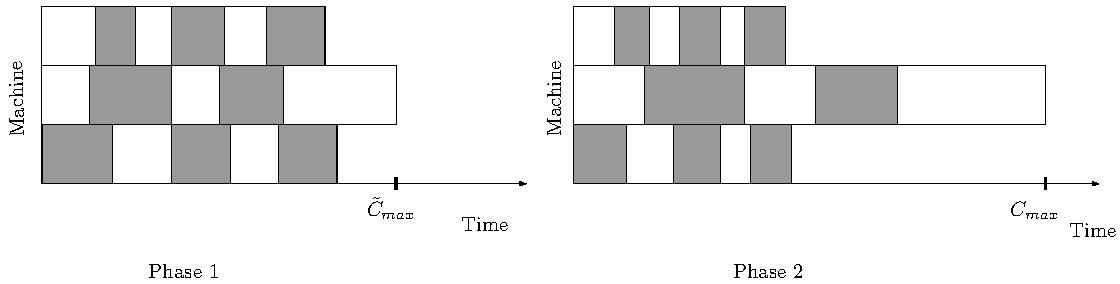
\includegraphics[width= 16 cm]{mem2.pdf}
                    \caption{An example of two phases of the schedule generated by the $SABO_\triangle$. The uncolored parts  represent tasks scheduled according $\pi_2$. The colored parts represents tasks scheduled according $\pi_1$}
                    \label{fig:ch5-1}
                    \end{figure} 
                      \begin{algorithm}                    
                      \caption{$SABO_\triangle$}
                      \label{alg2}
                       \begin{algorithmic} 
                       \State \textbf{Input:} $m$ machines 
                       \State \hspace*{42pt}Set $J$ of $n$ tasks
                       \State\hspace*{42pt}Let $\pi_1$ be a $ \rho_1$-approximated schedule on makespan $\tilde{C}_{max}$ 
                      \State \hspace*{42pt}Let $\pi_1$ be a $\rho_2$- approximated schedule on memory ${M_{max}}$
                      \State
                       \State \textbf{Phase 1:} [Uses $SBO_\triangle$]
                    \ForAll{$j\in S_1$}
                    \If{$\frac{\tilde{p_j}}{\tilde{C}^{\pi_1}_{max}} \leq \triangle \frac{s_j}{M^{\pi_2}_{max}}$}
                    \State Assign $j$ to a machine according to $\pi_2$ schedule
                    \State Add $j$ to $S_2$
                    \Else
                    \State Assign $j$ to a machine according to $\pi_1$ schedule
                    \State Add $j$ to $S_1$   
                    \EndIf 
                    \EndFor
                   
                     \State \textbf{End of Phase 1} 
                     \State 
                      \State \textbf{Phase 2:} 
                      \State \hspace*{42pt}Schedule tasks to machines to which they were assigned during phase 1
                         
                      \State \textbf{End of Phase 2} 
                       
                            \end{algorithmic}
                            \end{algorithm}     
        
                          
                         
                         \begin{theorem}
                         \label{th:chapter5-2a}
                          The $SABO_\triangle$ Algorithm generates a $(1+\triangle)\alpha^2 \rho_1$ - approximated schedule on makespan.
                         \end{theorem}         
                         \begin{proof}
                         Let $k$ be the machine reaching the makespan $C_{max}$ of the schedule. $C_{max}$ can be written as the sum of processing times of tasks in set $S_1$ and $S_2$ scheduled on machine $k$.
                         \begin{equation}\nonumber
                   C_{max}= \sum_{j \in S_1 \cap E_k}^{}p_j+\sum_{j \in S_2 \cap E_k}^{}p_j 
                         \end{equation}
                         
                         Since, $\sum\limits
                         _{j \in S_2 \cap E_k}^{}p_j\leq\alpha\sum\limits
                         _{j \in S_2 \cap E_k} \tilde{p}_j$
                           \begin{equation}\nonumber
                           C_{max} \leq \sum_{j \in S_1 \cap E_k}^{}p_j+\alpha\sum_{j \in S_2 \cap E_k} \tilde{p}_j 
                                 \end{equation}
                        
                         
                         Let $C^{\pi_1}_{max}$ denotes the makespan obtained after phase 2 when tasks are loaded and actual processing time of a task is known to scheduler. Since $C^{\pi_1}_{max} \geq \sum\limits
                         _{j \in S_1 \cap E_k}^{}p_j$ and $\sum\limits
                         _{j \in S_2\cap E_k}\triangle {\tilde{C}^{\pi_1}_{max}} \frac{s_j}{M^{\pi_2}_{max}}\geq \sum\limits
                         _{j \in S_2\cap E_k}^{}\tilde{p}_j $ by definition of $S_2$, we have
         \begin{equation}\nonumber
     C_{max}\leq C^{\pi_1}_{max}+\alpha\sum_{j \in S_2\cap E_k}^{}\triangle {\tilde{C}^{\pi_1}_{max}} \frac{s_j}{M^{\pi_2}_{max}}
                                \end{equation}                    
       Since, $C^{\pi_1}_{max}\leq\alpha\tilde{C}^{\pi_1}_{max}$ and $\sum\limits_{j \in S_2\cap E_k} \frac{s_j}{M^{\pi_2}_{max}}\leq 1$, we have
         \begin{equation}\nonumber                       C_{max}\leq(1+\triangle)\alpha\tilde{C}^{\pi_1}_{max}                         \end{equation}
      
     Since $ \tilde{C}^{\pi_1}_{max} \leq \rho_1 \tilde{C}^{*}_{max}\leq \alpha\rho_1 {C}^{*}_{max}$ the algorithm has an approximation ratio of $(1+\triangle)\alpha^2 \rho_1$ on makespan.
                             \end{proof}
   \begin{theorem} \label{th:chapter5-2b}
     The $SABO_\triangle$ Algorithm generates $ (1+\frac{1}{\triangle})\rho_2 $- approximated schedule on memory 
      \end{theorem}                      
      \begin{proof}  
      The proof is identical to $SBO_\triangle$ algorithm and is presented in chapter~\ref{ch3}.                                           
      \end{proof}    
 
 \bodysection{The $ABO_\triangle$ Algorithm} 
 We propose a two phase algorithm. In phase 1 the algorithm assigns tasks to all the machines such that it minimizes both the makespan as well as memory consumption. The tasks having more memory value  in comparison to its processing time are scheduled using memory intensive schedule which aim at minimizing memory.  Similarly tasks which incur more processing time cost compared to memory cost are assigned to machines according to the makespan intensive schedule. These   tasks are replicated to all machines in order to provide better load balancing and hence minimized makespan. The algorithm in its phase 1 assigns all the memory intensive tasks to machines first, then chooses tasks having more processing time values compared to memory they consume.
 
 In phase 2, the algorithm loads the memory intensive  tasks to the machines they were assigned in phase 1 respecting the tasks assignment during phase 1. The algorithm schedule the time intensive tasks (replicated tasks) using Graham's List Scheduling after all the memory intensive tasks are scheduled. Figure~\ref{fig:ch5-2} shows a schedule instance using the algorithm.\\
 
   \begin{figure}[htp]
   \centering
   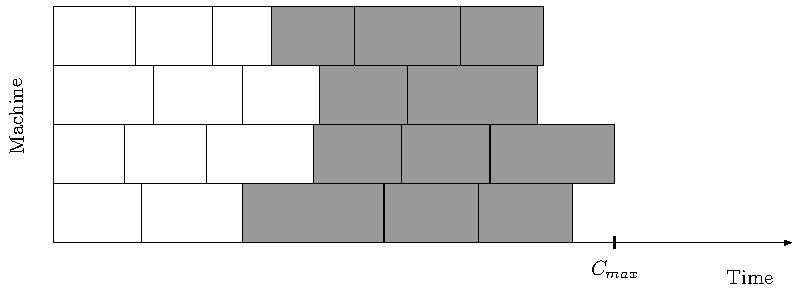
\includegraphics[width= 16 cm]{mem.pdf}
   \caption{An example of the schedule generated by the $ABO_\triangle$ algorithm. The uncolored parts represent the memory intensive tasks scheduled according $\pi_2$. The colored parts represent the processing time intensive tasks and scheduled using LS after replicated}
   \label{fig:ch5-2}
   \end{figure}
  \begin{algorithm}
  
  \caption{$ABO_\triangle$}
  \label{alg1}
   \begin{algorithmic} 
   \State \textbf{Input:} $m$ machines 
   \State \hspace*{42pt}Set $J$ of $n$ tasks
   \State\hspace*{42pt}Let $\pi_1$ be a $ \rho_1$-approximated schedule on makespan $\tilde{C}_{max}$ 
  \State \hspace*{42pt}Let $\pi_2$ be a $\rho_2$- approximated schedule on memory ${M_{max}}$
  \State
   \State \textbf{Phase 1:}
\ForAll{$j\in J$}
\If{$\frac{\tilde{p_j}}{\tilde{C}^{\pi_1}_{max}} \leq \triangle \frac{s_j}{M^{\pi_2}_{max}}$}
\State Assign $j$ to a machine according to $\pi_2$ schedule
\State Add task $j$ to set $S_2$   
\EndIf 
\EndFor
\ForAll{$j\in S_1$}
\If{$\frac{\tilde{p_j}}{\tilde{C}^{\pi_1}_{max}} \geq \triangle \frac{s_j}{M^{\pi_2}_{max}}$}
\State Add $j$ to set $S_1$
\State Replicate $j$ everywhere   
\EndIf 
\EndFor
 \State \textbf{End of Phase 1} 
 \State 
  \State \textbf{Phase 2:} 
  \State \hspace*{42pt}Schedule tasks from set $S_2$ respecting job assignment during phase 1
     \State \hspace*{42pt} Schedule all replicated tasks from set $S_1$ using Graham's LS Algorithm 
  \State \textbf{End of Phase 2} 
   
        \end{algorithmic}
        \end{algorithm}
      
        \begin{theorem}
        \label{th:chapter5-la}
         The $ABO_\triangle$ Algorithm  generates a $ (2-\frac{1}{m}+\triangle\alpha^2 \rho_1) $- approximated schedule on makespan.
        \end{theorem}         
        \begin{proof}
        Let $k$ be the machine reaching the makespan $C_{max}$ of the schedule. $C_{max}$ can be written as the sum of the processing times of tasks in sets $S_1$ and $S_2$ scheduled on machine $k$.
        \begin{equation}\nonumber
  C_{max}= \sum_{j \in S_1 \cap E_k}^{}p_j+\sum_{j \in S_2 \cap E_k}^{}p_j 
        \end{equation}
        
        Since, $\sum\limits
        _{j \in S_2 \cap E_k}^{}p_j\leq\alpha\sum\limits
        _{j \in S_2 \cap E_k} \tilde{p}_j$
          \begin{equation}\nonumber
          C_{max} \leq \sum_{j \in S_1 \cap E_k}^{}p_j+\alpha\sum_{j \in S_2 \cap E_k} \tilde{p}_j 
                \end{equation}
       
        
        Let $C^R_{max}$ denotes makespan obtained by scheduling the replicated tasks using LS. Since $C^R_{max} \geq \sum\limits
        _{j \in S_1 \cap E_k}^{}p_j$ and $\sum\limits
        _{j \in S_2\cap E_k}\triangle {\tilde{C}^{\pi_1}_{max}} \frac{s_j}{M^{\pi_2}_{max}}\geq \sum\limits
        _{j \in S_2\cap E_k}^{}\tilde{p}_j $ by definition of $S_2$, we have
        \begin{equation}\nonumber
         C_{max}\leq C^R_{max}+\alpha\sum_{j \in S_2\cap E_k}^{}\triangle {\tilde{C}^{\pi_1}_{max}} \frac{s_j}{M^{\pi_2}_{max}}
               \end{equation}
         Using the property of LS, the approximation ratio of the schedule incorporating only replicated tasks is $2-\frac{1}{m}$. So, $C^R_{max} \leq (2-\frac{1}{m})C^{*}_{max}$. Also, $\sum\limits
         _{j\in S_2\cap E_k}^{} \frac{s_j}{M^{\pi_2}_{max}}\leq 1$. 
         \begin{equation}\nonumber
                 C_{max}\leq (2-\frac{1}{m})C^{*}_{max}+\alpha\triangle {\tilde{C}^{\pi_1}_{max}} 
                       \end{equation}
            Also,  ${\tilde{C}^{\pi_1}_{max}} \leq \rho_1 {\tilde{C}^{*}_{max}}$. Since $\tilde{C}^{*}_{max}$ is the optimal makespan obtained after phase 1 considering estimated processing times of the tasks, we have, $\tilde{C}^{*}_{max}\leq \alpha{C}^{*}_{max}$. So, ${\tilde{C}^{\pi_1}_{max}} \leq \alpha \rho_1{C}^{*}_{max}$. Using this, we have         
           \begin{equation}\nonumber
                         C_{max}\leq (2-\frac{1}{m}){{C}^{*}_{max}}+\alpha^2\triangle \rho_1 {{C}^{*}_{max}} 
                               \end{equation}
            Hence, we proved that the algorithm generates a $(2-\frac{1}{m}+\triangle \alpha^2\rho_1) $- approximated schedule on makespan.
            \end{proof}
            \begin{theorem}
                   \label{th:chapter5-lb}
                    The $ABO_\triangle$ Algorithm generates a $ (1+\frac{m}{\triangle})\rho_2 $- approximated schedule on memory.
                   \end{theorem}
     
          \begin{proof}           
          When a task is replicated all its replica occupies space in memory and increase memory consumption. For $m$ replicas the total memory consumption is $m$ times of the replicated tasks. Similar to proof of previous theorem, the highest maximum memory occupied by any machine $k$ can be written as
           \begin{equation}\nonumber
           M_{max}= \sum_{j \in S_1\cap E_k}^{}s_j+\sum_{j \in S_2\cap E_k}^{}s_j           
        \end{equation}
        As each task in set $S_1$ is replicated over all the machines,$\sum\limits
        _{j \in S_1\cap E_k}^{}s_j =\sum\limits
        _{j \in S_1}^{}s_j$.              
            \begin{equation}\nonumber
                       M_{max} = \sum_{j\in S_1}^{}s_j+\sum_{j \in S_2\cap E_k}^{}s_j           
                    \end{equation}    
                     $\sum\limits_{j \in S_2\cap E_k}^{}s_j$  at most be equal to $M^{\pi_2}_{max} $ and $\sum\limits_{j\in S_1}s_j$ is bounded by $\sum\limits_{j \in J}^{} {M^{\pi_2}_{max}} \frac{\tilde{p_j}}{\triangle \tilde{C}^{\pi_1}_{max}} $ as per condition for  $\pi_1$ scheduling, using this we have    
 \begin{equation}\nonumber
 M_{max}\leq \sum_{j \in J}^{} {M^{\pi_2}_{max}} \frac{\tilde{p_j}}{\triangle \tilde{C}^{\pi_1}_{max}}+{M^{\pi_2}_{max}}
  \end{equation}
          Since $ \sum\limits_{j \in J}\tilde{p}_j \leq m\tilde{C}^{\pi_1}_{max} $, we have 
              \begin{equation}\nonumber
  M_{max}\leq   \frac{m}{\triangle}{M^{\pi_2}_{max}}+{M^{\pi_2}_{max}}
\end{equation}
 Also,  ${M^{\pi_2}_{max}} \leq \rho_2 {M^{*}_{max}}$.  Hence, The Algorithm generate $ (1+\frac{m}{\triangle})\rho_2 $- approximated schedule on memory.
               \end{proof}
               
               
 \bodysection{Summary}
  Table~\ref{tab:template2} summarizes the results for $SABO_\triangle$ and $ABO_\triangle$ algorithms. $SABO_\triangle$ is  similar to $ SBO_\triangle$ algorithm in its first phase and has a  approximation ratio of $[(1+\triangle)\alpha^2 \rho_1, (1+\frac{1}{\triangle})\rho_2]$ on makespan and memory.   $ABO_\triangle$ is a $ [(2-\frac{1}{m}+\triangle\alpha^2 \rho_1), (1+\frac{m}{\triangle})\rho_2] $-approximated algorithm on makespan and memory and replicate processing time intensive tasks to improve makespan.\\
  \\
  
  \begin{table}[ht]
      \centering
      \begin{tabular}{|l|c|c|c|c|c|}
        \hline
        Algorithm & Approx. on makespan & Approx. on memory  \\
        \hline
        $SABO_\triangle$&
        $(1+\triangle)\alpha^2 \rho_1$ (Th.~\ref{th:chapter5-2a})& $(1+\frac{1}{\triangle})\rho_2$ (Th.~\ref{th:chapter5-2b})   \\
        \hline
                $ABO_\triangle$&
                $(2-\frac{1}{m}+\triangle\alpha^2 \rho_1$ (Th.~\ref{th:chapter5-la})& $(2-\frac{1}{m}+\triangle\alpha^2 \rho_1)$ (Th.~\ref{th:chapter5-lb})   \\
        
        
        
    %    & $\frac{C_{max}}{C_{max}^{*}} \leq  1+ \frac{2}{1+\alpha^{2}} \left(\alpha^2-\frac{1}{m}\right)$ when $k=2$ [Col. 3.1]   \\
        
        \hline
      \end{tabular}
      \caption{Summary of the results of $SABO_\triangle$ and $ABO_\triangle$.}
      \label{tab:template2}
    \end{table}
  
  
   \begin {figure}
      \centering
      \begin{subfigure}[b]{0.5\textwidth}
        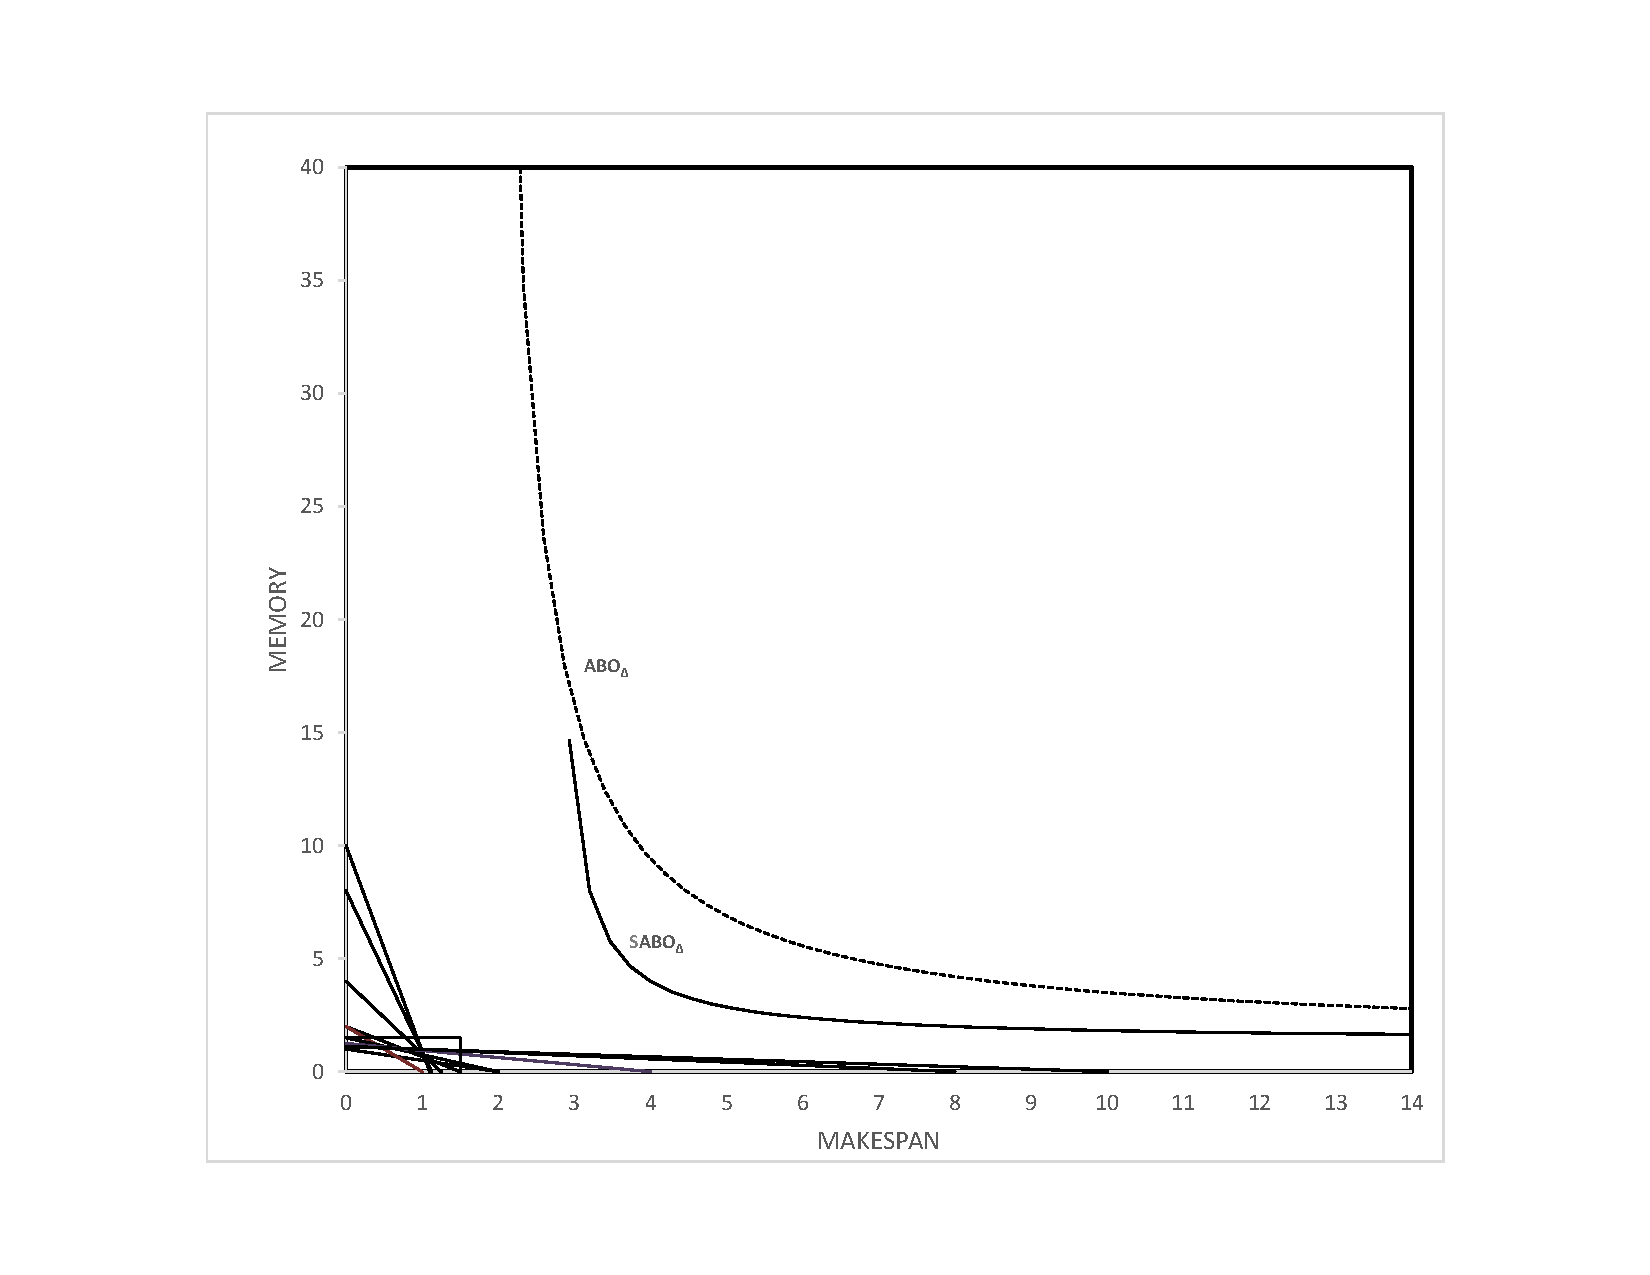
\includegraphics[width=\textwidth]{graph_M5_ALPHAsq_2.pdf}
        \caption{$m=5$, $\alpha^2=2$, $\rho_1=\rho_2=4/3$}
        \label{fig:ch5-3.1}
      \end {subfigure} %
      
      \begin{subfigure}[b]{0.5\textwidth}
        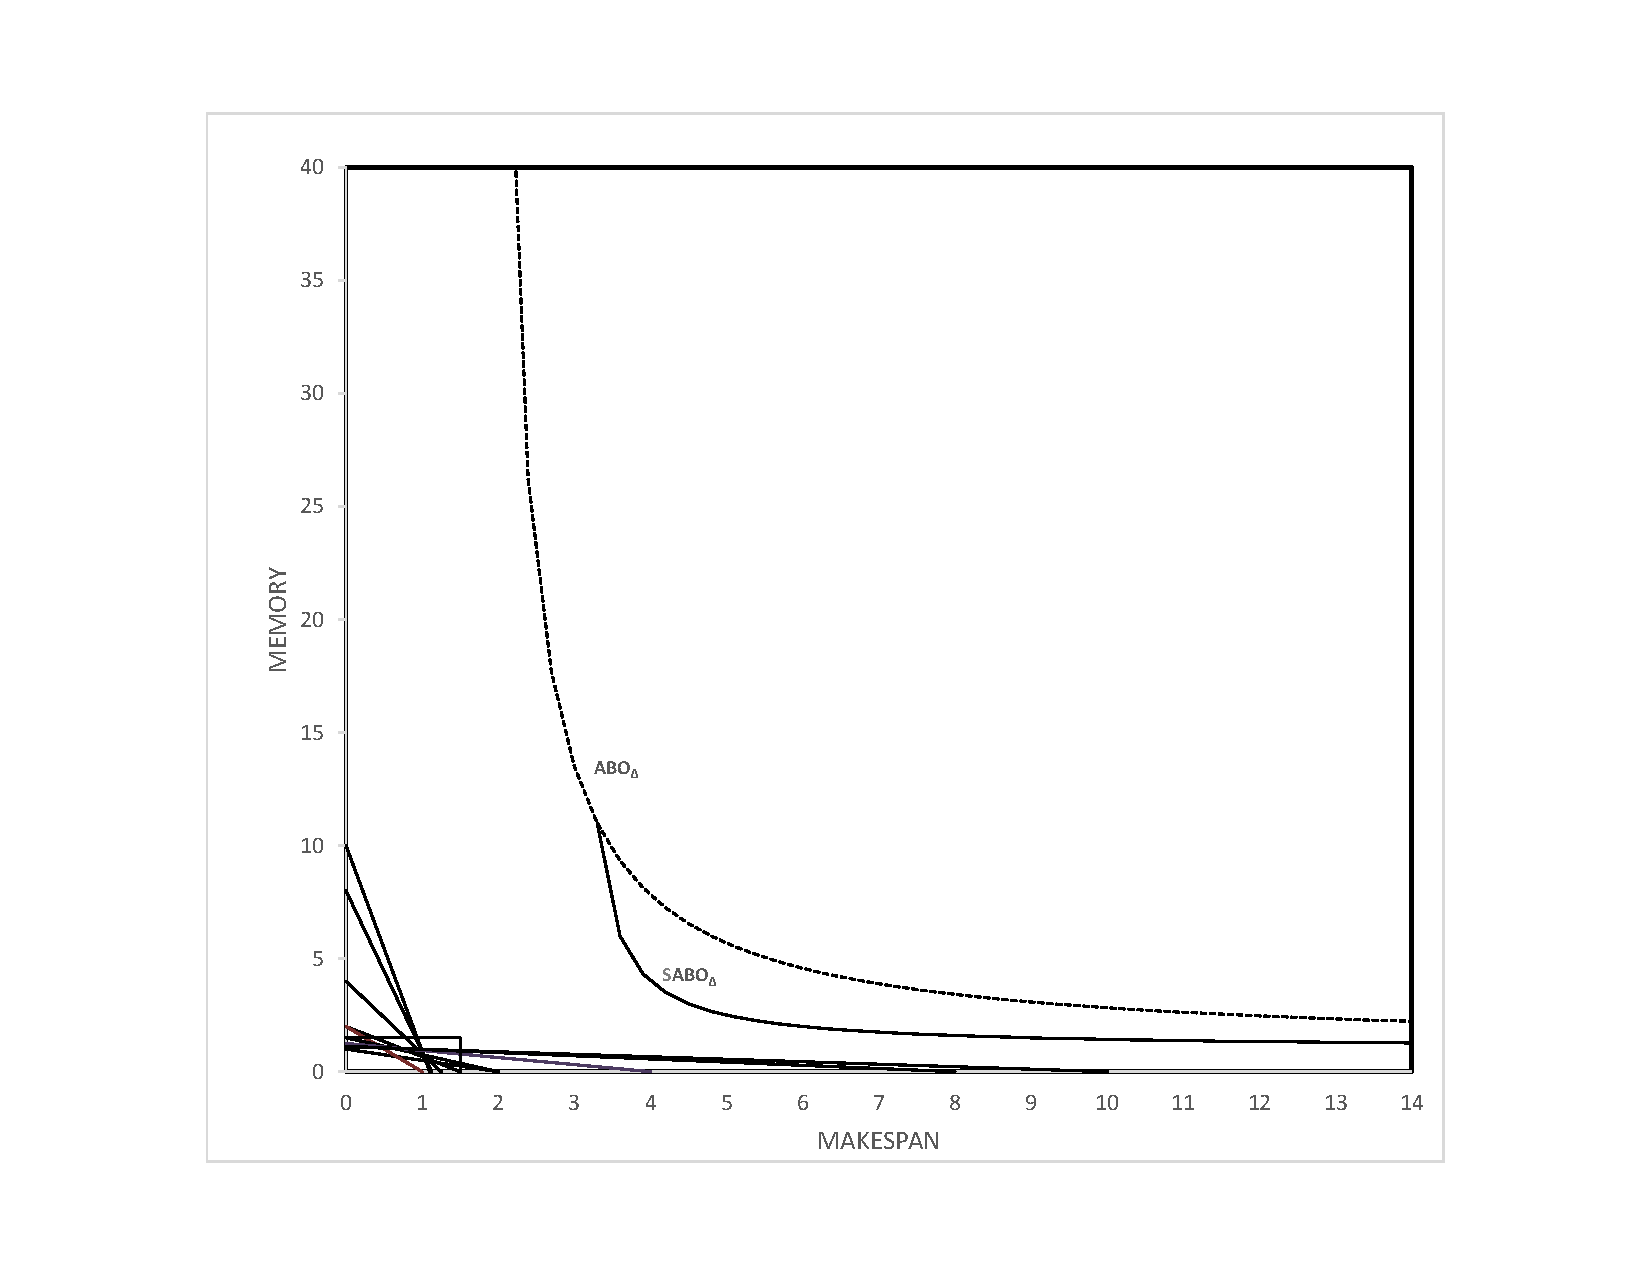
\includegraphics[width=\textwidth]{graph_M10_ALPHsq_3_rho_1.pdf}
        \caption{$m=5$, $\alpha=3$, $\rho_1=\rho_2=1$}
        \label{fig:ch5-3.2}
      \end {subfigure} %
      
      \begin{subfigure}[b]{0.5\textwidth}
        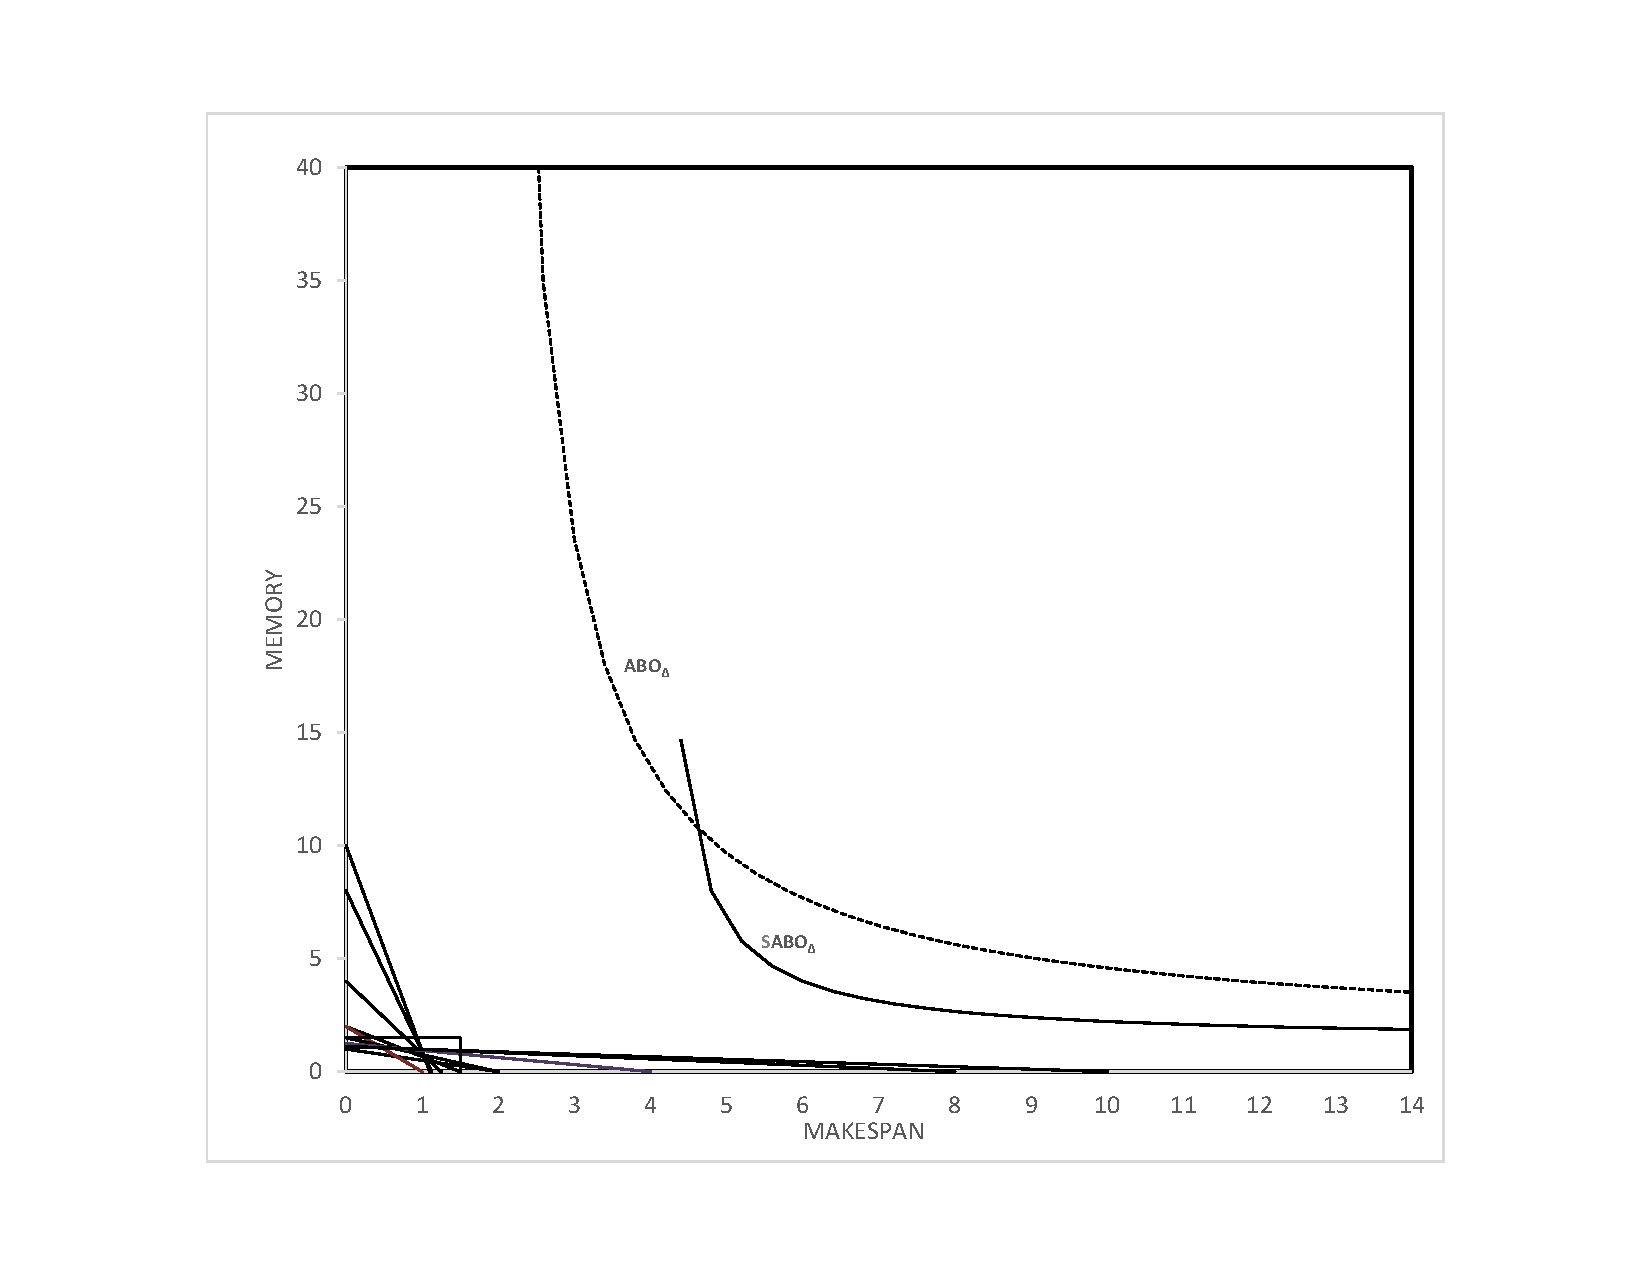
\includegraphics[width=\textwidth]{graph_M10_ALPHsq_3_rho_133.pdf}
        \caption{$m=5$, $\alpha=3$, $\rho_1=\rho_2=4/3$}
        \label{fig:ch5-3.3}
      \end{subfigure} %
    
      \caption{Memory-Makespan graph for $SABO_\triangle$ and $ABO_\triangle$. The bold lines represent impossibilities in tradeoff between guarantees.}
      \label{fig:ch5-3}
    \end{figure}\
    
 To better understand the tradeoff between memory consumption and makespan Figure~\ref{fig:ch5-3} shows memory-makespan graph for the two algorithms. The graph shows that for higher values for $\alpha$ the  algorithm $ABO_\triangle$ have better tradeoff between memory-makespan than that of  $SABO_\triangle$. for $\alpha\rho_1\geq 2$,  $ABO_\triangle$ always have better guarantee on makespan than $SABO_\triangle$. So, a schedule more centric to optimize makespan should follow $ABO_\triangle$ algorithm. And a memory centric schedule should follow $SABO_\triangle$ as the algorithm always has better guarantee on memory.
 
 The bold lines shows impossibilities in the tradeoff between makespan and memory and means that no algorithm can guarantee better tradeoff than this. \cite{10.1109/IPDPS.2008.4536292} discusses about these impossibilities in context of $SBO_\triangle$ algorithm.
 
  
              
               
               
        